%!TEX root=../GaugeCNNTheory.tex


\subsection{گیج‌ها، تبدیل‌های گیج و \textit{$G$}-ساختارها}
\label{sec:21_main}


\subsubsection{فضاهای مماس و چارچوب‌های مرجع}
\label{sec:gauges_gauge_trafos}


یک منیفولد هموار $d$ -بعدی $M$ دارای یک فضای مماس $\TpM\cong\R^d$ متصل به هر نقطه $p\in M$ است. فضاهای مماس، فضاهای برداری $d$-بعدی هستند، با این حال، برخلاف $\R^d$، آن‌ها به طور کلی با هیچ انتخاب ارجح چارچوب مرجع همراه نیستند. یک بردار مماس $v\in \TpM$ یک شی \emph{مستقل از مختصات} است و بنابراین بلافاصله به صورت عددی با یک تاپل مختصاتی $(v_1,\dots,v_d)\in\R^d$ نمایش داده نمی‌شود. به طور انتزاعی‌تر، هر فضای مماس $\TpM$ با~$\R^d$ هم‌ریخت است اما به طور کلی هیچ هم‌ریختی کانونی بین آن‌ها وجود ندارد. بنابراین هر دو فضا از نظر ساختاری معادل هستند اما به هیچ روش ارجح به یکدیگر شناسایی نمی‌شوند.


یک \emph{گیج} (تسهیم محلی بندل مماس) بر روی $U^A\subseteq M$ به عنوان مجموعه‌ای از نگاشت‌های خطی معکوس‌پذیر که به صورت هموار وابسته به موقعیت هستند، تعریف می‌شود:
\begin{align}\label{eq:gauge_definition}
	\psi_p^A:\TpM\to\R^d \,,\ \ p\in U^A \,,
\end{align}
که هم‌ریختی‌های فضای برداری گمشده بین $\TpM$ و $\R^d$ را مشخص می‌کند. همانطور که در شکل~\ref{fig:gauge_trafos} بصری‌سازی شده است، آن‌ها با تخصیص یک \emph{بردار ضریب} به فضاهای مماس مختصات می‌دهند:
\begin{align}
	v^A\ :=\ \psi_p^A(v) \ \in\R^d
\end{align}
به هر بردار مماس مستقل از مختصات $v\in \TpM$. معکوس این رابطه می‌دهد:
\begin{align}
	v\ =\ \left(\psi_p^A\right)^{-1}\! (v^A)
	\ =\ \left(\psi_p^A\right)^{-1}\!\! \left(\sum\nolimits_i v_i^A \epsilon_i\right)
	\ =\ \sum\nolimits_i v_i^A\, \left(\psi_p^A\right)^{-1}\!(\epsilon_i)
	\ =:\ \sum\nolimits_i v_i^A\, e_i^A \,,
\end{align}
که در آن $\{\epsilon_1,\dots,\epsilon_d\}$ را پایانه استاندارد $\R^d$ نامگذاری کرده‌ایم و از خطی بودن گیج برای بیرون کشیدن جمع استفاده کرده‌ایم. این نشان می‌دهد که گیج را می‌توان به عنوان مجهز کردن هر فضای مماس $\TpM$ با یک \emph{چارچوب مرجع} در نظر گرفت:
\begin{align}\label{eq:framefield_gauge_equivalence}
	\left[e^A_{1}, \,\dots,\, e^A_{d}\right]
	\ :=\ \Big[(\psi_p^A)^{-1}(\epsilon_1), \:\dots\,,\; (\psi_p^A)^{-1}(\epsilon_d)\Big] \,,
\end{align}
که به عنوان یک \lr{d}-تاپل از بردارهای مماس خطی مستقل تعریف می‌شود که با نگاشت پایه استاندارد $\R^d$ به عقب از طریق نگاشت معکوس گیج به دست می‌آید. برای اختصار، ما در ادامه از نماد کوتاه‌شده $\big[e_i^A \big]_{i=1}^d$ برای چارچوب‌ها $\big[e_1^A, \dots, e_d^A \big]$ استفاده خواهیم کرد. ضرایب $v^A$ مختصات $v$ نسبت به این چارچوب هستند. مجموعه‌ای از چارچوب‌های القا شده توسط $\psi_p^A$ بر روی $U^A$ (هموار) \emph{میدان چارچوب} نامیده می‌شود؛ برای بصری‌سازی به شکل~\ref{fig:gauge_trafos_manifold} مراجعه کنید.


\begin{figure}
	\centering
	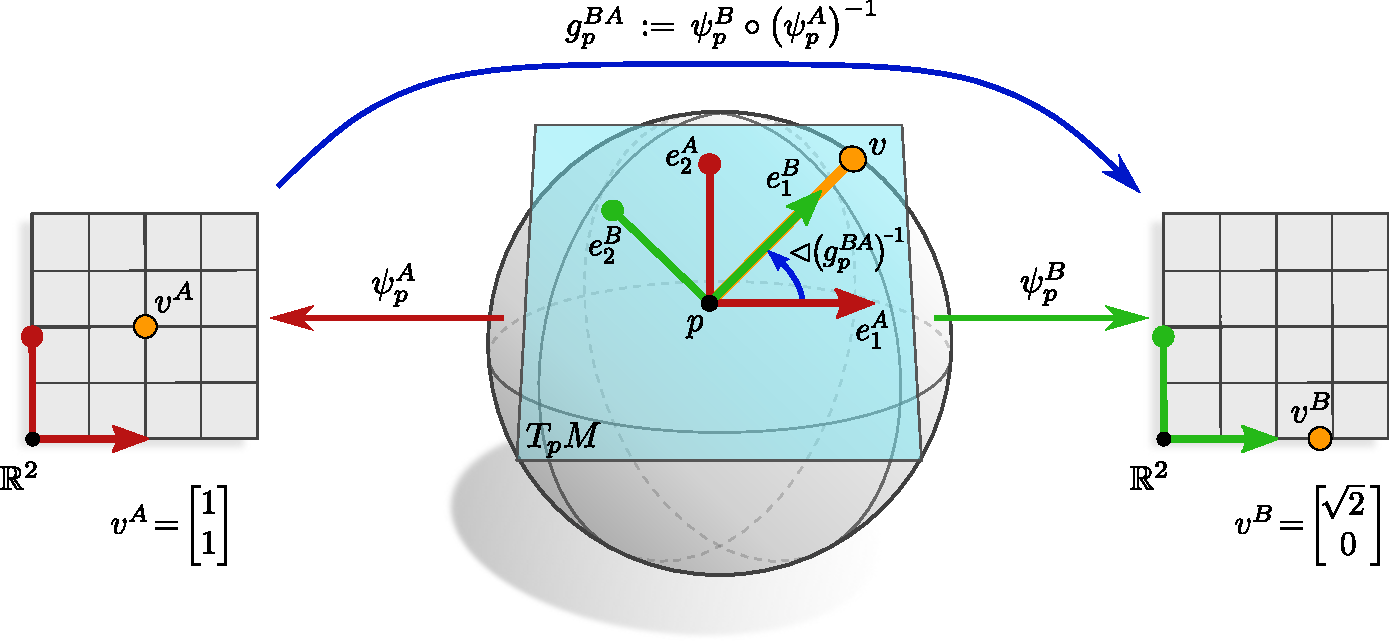
\includegraphics[width=\columnwidth]{figures/gauges_TpM.pdf}
	\caption{\small
		شناسایی $\TpM\!\cong\!\R^2$ با $\R^2$ از طریق گیج‌های مختلف.
		یک بردار مماس (مستقل از مختصات) $v\in \TpM$ (نارنجی) را می‌توان به صورت عددی با یک تاپل مختصاتی $v^A=\psi_p^A(v)=\big(1,1\big)^\top$ نسبت به گیج $\psi_p^A$ (قرمز) یا، به طور معادل، با $v^B=\psi_p^B(v)=(\sqrt{2},0)^\top$ نسبت به گیج $\psi_p^B$ (سبز) نمایش داد.
		انتخاب یک گیج مربوط به انتخاب $[e_1^A,e_2^A]$ یا $[e_1^B,e_2^B]$ از چارچوب مرجع است.
		در یک منیفولد عمومی هیچ انتخابی از گیج یا مختصات‌بندی پیش‌فرض ارجح نیست.
		گیج‌های مختلف، و در نتیجه چارچوب‌های مرجع، با تبدیل‌های گیج $g_p^{BA}:=\psi_p^B\circ(\psi_p^A)^{-1}$ (آبی) مرتبط هستند که مقادیری در گروه ساختار $G$ تعریف شده می‌گیرند.
		این شکل تفسیری گرافیکی از نمودارهای جابجایی در معادله~\eqref{eq:commutative_diagram_TpM} و شکل~\ref{fig:trivialization_TM} است.
		توجه داشته باشید که گیج‌ها بلافاصله به فضاهای مماس مختصات می‌دهند.
		شکل~\ref{fig:affine_charts} در بخش~\ref{sec:euclidean_geometry} یک نمودار مشابه برای چارت‌های (آفین) را نشان می‌دهد که به منیفولد مختصات می‌دهند و بدین ترتیب گیج‌ها ("پایه‌های مختصات") را \emph{القا} می‌کنند.
	}
	\label{fig:gauge_trafos}
\end{figure}


گیج‌های $\psi^X$ فضاهای مماس را تنها در همسایگی‌های محلی $U^X\subseteq M$ مختصات می‌دهند، و به دلیل موانع توپولوژیکی به طور کلی نمی‌توانند به کل منیفولد بدون نقض فرض همواری گسترش یابند.
بنابراین یک \emph{اطلس} در نظر گرفته می‌شود:
\begin{align}
	\mathscr{A} \,=\, \big\{\! \big(U^X, \psi^X\big) \!\big\}_{X\in \mathfrak{X}} \,,
\end{align}
متشکل از گیج‌های هموار بر روی مجموعه‌ای از همسایگی‌های $U^X$ که منیفولد را پوشش می‌دهند، یعنی شرط $\bigcup_{X\in \mathfrak{X}} U^X = M$ را برآورده می‌کنند، که در آن $\mathfrak{X}$ یک مجموعه اندیس است.%
\footnote{
	اطلس گیج‌ها بسیار شبیه به اطلس‌های معمول چارت‌های یک منیفولد است (پیوست~\ref{apx:coordinate_bases}).
	تفاوت این است که اطلس‌های مورد نظر در اینجا مستقیماً به بندل مماس $\TM$ مختصات می‌دهند به جای منیفولد $M$.
}
در نواحی همپوشانی $U^A\cap U^B\neq\varnothing$ از همسایگی‌ها، گیج‌های مختلف $\psi_p^A$ و $\psi_p^B$ توسط \emph{توابع گذار} هموار به هم متصل می‌شوند:
\begin{align}\label{eq:transition_fct_local_def_21}
	g^{BA}\!:\, U^A\cap U^B\to\GL{d},\quad p \mapsto g_p^{BA} := \psi_p^B \circ \left(\psi_p^A\right)^{-1}.
\end{align}
در اینجا ما دامنه مشترک (فعلاً) را با \emph{گروه خطی عمومی} $\GL{d}$ در نظر می‌گیریم، متشکل از همه ماتریس‌های معکوس‌پذیر در $ \R^{d\times d}$، که رابطه بین هر جفت از هم‌ریختی‌های فضای برداری (گیج‌ها) یا چارچوب‌های مرجع را توضیح می‌دهند.
عمل چنین تابع گذاری بر روی یک گیج داده شده یک \emph{تبدیل گیج} را تعریف می‌کند:
\begin{align}\label{eq:gauge_trafo_local_def_21}
	\psi_p^B\ =\ g_p^{BA} \!\cdot \psi_p^A.
\end{align}
از نظر یک نمودار جابجایی، رابطه بین گیج‌های مختلف به صورت زیر بصری‌سازی می‌شود:%
\footnote{
	\mbox{
		\emph{نمودارها} یک نمای کلی بصری از توابع و فضاهایی را که بین آن‌ها نگاشت می‌کنند، ارائه می‌دهند.
		به عنوان مثال، نمودار
	}
	\begin{minipage}{.2\textwidth}
		${
			\mkern30mu
			\begin{tikzcd}[column sep=30pt, row sep=8pt, ampersand replacement=\&]
				X
				\arrow[r, pos=.55, "f" description]
				\arrow[rd, "h\!"']
				\& Y
				\arrow[d, "\;g"]
				\\
				\& Z
		\end{tikzcd}}$
	\end{minipage}
	\hfill
	\begin{minipage}{.8\textwidth}
		به این معنی است که توابع $f:X\to Y$، \ $g:Y\to Z$ و $h:X\to Z$ وجود دارند.
		اگر ترکیبات توابع در امتداد \emph{همه} مسیرهایی با شروع و پایان یکسان مطابقت داشته باشند، نمودار \emph{جابجایی} نامیده می‌شود.
		نمودار مثال ما اگر (و تنها اگر) \ $h = g\circ f$ صادق باشد، جابجایی است.
	\end{minipage}
}
\vspace*{-1ex}
\begin{equation}\label{eq:commutative_diagram_TpM}
	\begin{tikzcd}[column sep=50pt, row sep=5pt, font=\normalsize]
		\R^d
		\arrow[rr, rounded corners, to path={
			-- ([yshift=4.5ex]\tikztostart.north)
			--node[above, pos=.5]{\small$g_p^{BA} \mkern2mu\cdot$} ([yshift=4.5ex]\tikztotarget.north)
			-- (\tikztotarget.north)
		}]
		& \TpM
		\arrow[l, "\psi_p^A"']
		\arrow[r, "\psi_p^B"]
		& \R^d
		\arrow[ll, rounded corners, to path={
			-- ([yshift=-4.5ex]\tikztostart.south)
			--node[below, pos=.5]{\small$g_p^{AB} \mkern2mu\cdot \,=\, \big( g_p^{BA} \big)^{-1} \mkern2mu\cdot$} ([yshift=-4.5ex]\tikztotarget.south)
			-- (\tikztotarget.south)
		}]
	\end{tikzcd}
	\vspace*{-1ex}%
\end{equation}
این نمودار را با تفسیر گرافیکی آن در شکل~\ref{fig:gauge_trafos} مقایسه کنید.


یک تبدیل گیج، مختصات‌بندی فضاهای مماس را تغییر می‌دهد به طوری که همان بردار مماس مستقل از مختصات $v$ با یک بردار مولفه‌ای متفاوت نمایش داده می‌شود:
\begin{align}\label{eq:components_leftaction}
	v^B\ =\ g_p^{BA}v^A \,.
\end{align}
از آنجا که یک گیج مربوط به انتخاب یک میدان چارچوب است، یک تبدیل گیج مربوط به تبدیل بین میدان‌های چارچوب است.
به طور خاص، یک چارچوب $\big[e_i^A\big]_{i=1}^d = \big[e_1^A,\dots,e_d^A\big]$ در $p\in M$ به یک چارچوب دیگر تبدیل می‌شود:
\begin{alignat}{3}\label{eq:frame_rightaction}
	\qquad
	\left[e_{i}^B\right]_{i=1}^d\ \notag
	:=&\ \left[ \left(\psi_p^B\right)^{-1} (\epsilon_i) \right]_{i=1}^d
	\qquad\quad && \big( \text{\small چارچوب القا شده توسط گیج، معادله~\eqref{eq:framefield_gauge_equivalence} } \big) \notag\\
	=&\ \left[ \left(g_p^{BA} \cdot \psi_p^A\right)^{-1} \left(\epsilon_i\right) \right]_{i=1}^d
	\qquad\quad && \big( \text{\small تبدیل گیج، معادله~\eqref{eq:gauge_trafo_local_def_21}} \big) \notag\\
	=&\ \left[ \left(\psi_p^A\right)^{-1} \left(\left(g_p^{BA}\right)^{-1} \epsilon_i\right) \right]_{i=1}^d
	\qquad\quad && \big( \text{\small معکوس گسترش یافته} \big) \notag\\
	=&\ \left[ \left(\psi_p^A\right)^{-1} \left(\sum\nolimits_j \epsilon_j \epsilon_j^\top \left(g_p^{BA}\right)^{-1} \epsilon_i\right) \right]_{i=1}^d
	\qquad\quad && \big( \text{\small هویت وارد شده}\ {\textstyle\mathds{1}=\sum_j\epsilon_j\epsilon_j^\top}\ \big) \notag\\
	=&\ \left[ \left(\psi_p^A\right)^{-1} \left(\sum\nolimits_j \epsilon_j \left(\!\left(g_p^{BA}\right)^{-1}\right)_{ji} \right) \right]_{i=1}^d
	\qquad\quad && \big( \text{\small عناصر ماتریس $\big(g_p^{BA}\big)^{-1}$ شناسایی شده} \big) \notag\\
	=&\ \left[ \sum\nolimits_j \left(\psi_p^A\right)^{-1}\! (\epsilon_j)\ \left(\!\left(g_p^{BA}\right)^{-1}\right)_{ji} \right]_{i=1}^d
	\qquad\quad && \big( \text{\small خطی بودن $\psi_p^A$} \big) \notag\\
	=&\ \left[ \sum\nolimits_j e_{j}^A \left(\!\left(g_p^{BA}\right)^{-1}\right)_{ji} \right]_{i=1}^d
	\qquad\quad && \big( \text{\small چارچوب القا شده توسط گیج، معادله~\eqref{eq:framefield_gauge_equivalence} } \big) \notag\\
	=&\mkern-6mu: \left[ e_{i}^A \right]_{i=1}^d \btr \left(g_p^{BA}\right)^{-1}
	\qquad\qquad &&
\end{alignat}
از طریق \emph{عمل راست} تعریف شده:
\begin{align}\label{eq:right_action_mapsto}
	\btr:\ \pig( [e_i]_{i=1}^d,\ g \pig)\ \mapsto\ [e_i]_{i=1}^d \btr g\, :=\,  \Big[ \sum\nolimits_j e_j\, g_{ji} \Big]_{i=1}^d
\end{align}
از عناصر گروه بر روی چارچوب‌ها.
توجه داشته باشید که معکوس در این عمل در معادله~\eqref{eq:frame_rightaction} به دلیل تعریف معادله~\eqref{eq:gauge_trafo_local_def_21} بدون معکوس است.%
\footnote{
	قراردادهای دیگر ممکن است انتخاب معکوس‌ها را در
	$\psi^B = g^{BA}\psi^A$ و $[e_i^B]_{i=1}^d = [e_i^A]_{i=1}^d\btr \big(g^{BA}\big)^{-1}\!$ تغییر دهند.
	یک معکوس در هر یک از دو معادله برای سازگاری عمل چپ $\cdot$ بر روی گیج‌ها و عمل راست $\btr$ بر روی چارچوب‌ها ضروری است.
}
معمولاً به رفتار تبدیل چارچوب‌های مرجع، تبدیل \emph{کوواریانت} گفته می‌شود در حالی که تبدیل گیج‌ها و ضرایب برداری به عنوان تبدیل \emph{کونترواریانت} نامیده می‌شود؛ به پیوست~\ref{apx:coordinate_bases} مراجعه کنید.

\begin{SCfigure}
	\centering
	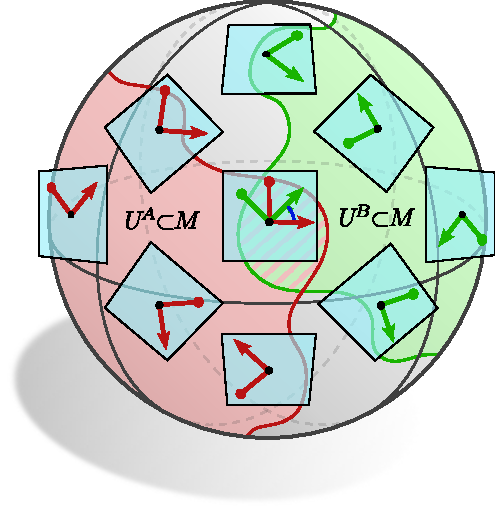
\includegraphics[width=.45\columnwidth]{figures/sphere_framefield.pdf}
	\captionsetup{width=.9\textwidth}
	\hspace{1ex}
	\caption{\small
		هر نقطه $p$ از یک منیفولد ریمانی $M$ دارای یک فضای مماس $\TpM$ متصل است.
		یک گیج هموار $\psi^A$ بر روی یک زیرمجموعه مناسب انتخاب شده $U^A \subseteq M$ (قرمز) تمام فضاهای مماس $\TpM$ را برای $p$ در $U^A$ مختصات می‌دهد همانطور که در شکل~\ref{fig:gauge_trafos} نشان داده شده است.
		این معادل انتخاب یک \emph{میدان چارچوب هموار} بر روی $U^A$ است.
		از آنجا که به طور کلی امکان گسترش یک گیج به صورت سراسری بر روی کل منیفولد وجود ندارد، لازم است که یک \mbox{$G$-\emph{اطلس}} در نظر گرفته شود، متشکل از گیج‌هایی که $M$ را پوشش می‌دهند.
		مختصات‌بندی‌های مختلف $\psi^A$ بر روی $U^A$ (قرمز) و $\psi^B$ بر روی $U^B$ (سبز) از طریق تبدیل‌های گیج (یا نگاشت‌های گذار) ${g^{BA}: U^A \cap U^B \to G}$ به هم متصل می‌شوند که بر روی همپوشانی ${U^A\cap U^B}$ (خط‌دار) تعریف شده‌اند و مقادیری در گروه ساختار $G \leq \GL{d}$ می‌گیرند.
		\\\protect\rule{0ex}{7.5ex}
	}
	\label{fig:gauge_trafos_manifold}
\end{SCfigure}


از آنجا که رفتار تبدیل ضرایب در معادله~\eqref{eq:components_leftaction} و پایه در معادله~\eqref{eq:frame_rightaction} معکوس یکدیگر هستند، آن‌ها یکدیگر را خنثی می‌کنند، یعنی بردار مماس $v = \sum_i v_i^A e_{i}^A = \sum_i v_i^B e_{i}^B$ را ناوردا می‌گذارند:
\begin{align}\label{eq:vector_in_different_bases}
	v\ =\ \sum\nolimits_i v_i^B e_{i}^B
	\ &=\ \sum\nolimits_i v_i^B \sum\nolimits_j e_{j}^A \left(\left(g_p^{BA}\right)^{-1}\right)_{ji} \notag\\
	\ &=\ \sum\nolimits_j \left(\sum\nolimits_i \left(\left(g_p^{BA}\right)^{-1}\right)_{ji} v_i^B\right) e_{j}^A \notag\\
	\ &=\ \sum\nolimits_j v_j^A e_{j}^A \,.
\end{align}
این ساختار تضمین می‌کند که هر محاسبه‌ای در نهایت مستقل از گیج انتخاب شده است، که معمولاً به آن \emph{استقلال از مختصات} گفته می‌شود. به طور کلی، هر نمایش مختصاتی از یک شی یا تابع مستقل از مختصات برای دلایل سازگاری باید مستقل از مختصات باشد.


برای کامل بودن می‌خواهیم اشاره کنیم که فرمالیسم ارائه شده در اینجا پایه‌های عمومی فضاهای مماس را تعریف می‌کند، که گاهی اوقات به عنوان \emph{پایه‌های غیرمختصاتی} (پایه‌های غیرهولونومیک) از نظر گیج‌های محلی نامیده می‌شوند.
یک جایگزین بسیار محبوب اما کمتر عمومی \emph{پایه‌های مختصاتی} (پایه‌های هولونومیک) هستند:
\begin{align}
	\bigg[\frac{\partial}{\partial x^A_1} \bigg|_p ,\,\dots\,,\ \frac{\partial}{\partial x^A_d} \bigg|_p \bigg] \,,
\end{align}
که توسط \emph{چارت‌های مختصاتی} منیفولد القا می‌شوند \cite{nakahara2003geometry}:
\begin{align}\label{eq:chart_21}
	x^A: U^A \to V^A \subseteq \R^d
\end{align}
گیج‌های مربوطه توسط \emph{دیفرانسیل‌های چارت} داده می‌شوند، یعنی:
\begin{align}
	\psi_p^A \,=\, \hat{d}x^A_p \,=\, \big( \hat{d}x^A_{p,1} \,,\dots,\, \hat{d}x^A_{p,d} \big)^\top\ :\ \TpM \to \R^d \,.
\end{align}
تبدیل‌های گیج در این تنظیم با \emph{ژاکوبیان‌ها} مطابقت دارند:
\begin{align}
	g_p^{BA} \,=\, \frac{\partial x^B}{\partial x^A} \bigg|_{x^A(p)} \,\in\, \GL{d}
\end{align}
از نگاشت‌های گذار چارت.
یک چارت نمونه و پایه‌های مختصاتی القا شده آن در شکل~\ref{fig:sphere_chart} بصری‌سازی شده‌اند.
پیوست~\ref{apx:coordinate_bases} رابطه بین هر دو فرمالیسم را با جزئیات مورد بحث قرار می‌دهد؛ یک مرور کلی در جدول~\ref{tab:coord_charts_gauge_trafos} ارائه شده است.


\begin{figure}
	\centering
	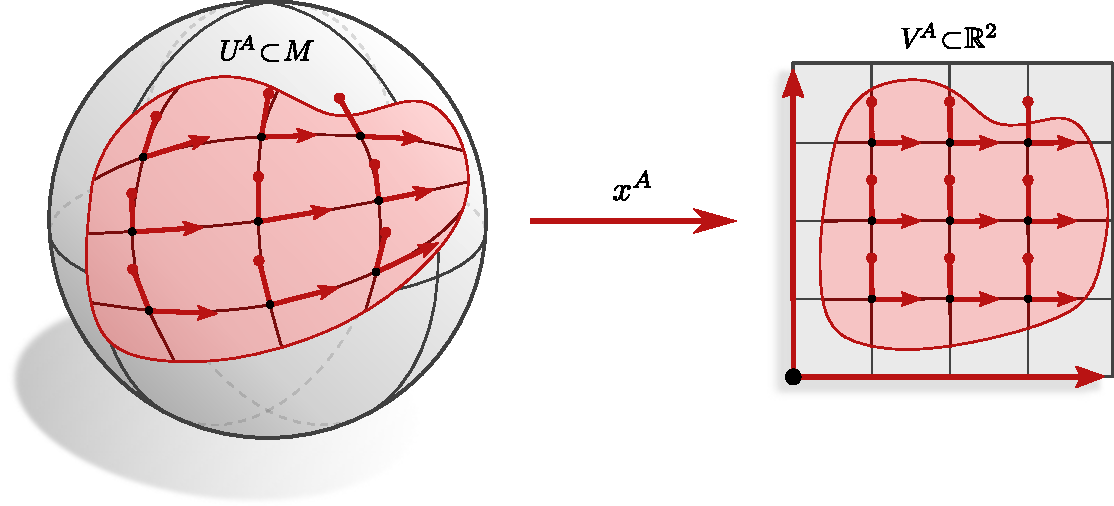
\includegraphics[width=.86\textwidth]{figures/sphere_chart.pdf}
	\hspace*{4ex}
	\caption{\small
		یک \emph{چارت} $x^A: U^A \to V^A$ مختصات $V^A \subseteq \R^d$ را به نواحی $U^A \subseteq M$ از منیفولد تخصیص می‌دهد.
		این چارت \emph{پایه‌های مختصاتی}
		$\big[\frac{\partial}{\partial x^A_1} \big|_p ,\,\dots\,,\ \frac{\partial}{\partial x^A_d} \big|_p \big]$
		و گیج‌های مربوطه $\psi_p^A = \hat{d}x_p^A$ را برای فضاهای مماس $\TpM$ در~$U^A$ القا می‌کند.
		ما عمدتاً با چارت‌ها کار نخواهیم کرد بلکه به نقاط $p\in M$ به صورت \emph{مستقل از مختصات} ارجاع خواهیم داد.
		گیج‌ها (چارچوب‌ها) سپس مستقیماً به فضاهای مماس تخصیص داده می‌شوند به جای اینکه از چارت‌ها القا شوند.
	}
	\label{fig:sphere_chart}
\end{figure}


در ادامه این مقاله ما عمدتاً در فرمالیسم گیج کار خواهیم کرد، که چارچوب‌های مرجع را مستقیماً به فضاهای مماس تخصیص می‌دهد به جای اینکه آن‌ها را از چارت‌ها القا کند.
استثناها عبارتند از
کانولوشن‌های موبیوس در بخش~\ref{sec:mobius_conv}،
\CNN{}های اقلیدسی در بخش~\ref{sec:instantiations_euclidean}،
مختصات لگاریتمی-قطبی در بخش~\ref{sec:polar_Euc2_logpolar}
و \CNN{}های بیست‌وجهی در بخش~\ref{sec:spherical_CNNs_icosahedral}.
در همه این موارد، منیفلدهایی \emph{به صورت محلی مسطح} هستند و چارت‌ها \emph{ایزومتریک} هستند، به طوری که \emph{چارچوب‌های متعامد} را القا می‌کنند.
کانولوشن‌های $\GM$ در $U^A$ سپس می‌توانند به روشی کارآمد با اجرای کانولوشن‌های اقلیدسی با کرنل‌های $G$-استیریبل در دامنه‌های مشترک چارت‌ها~$V^A$ محاسبه شوند.


\subsubsection{توابع مستقل از مختصات در فضاهای مماس}
\label{sec:gauges_TpM_functions}

همانطور که بردارهای $v\in \TpM$، \emph{توابع} بر روی فضاهای مماس مستقل از مختصات هستند، یعنی بدون اشاره به هیچ چارچوب مرجع تعریف می‌شوند.
یک گیج انتخاب شده امکان نمایش چنین نگاشت‌های مستقل از مختصات را توسط توابعی فراهم می‌کند که بر روی بردارهای ضریب در $\R^d$ عمل می‌کنند.
مشابه بردارهای ضریب، مختصات‌بندی توابع باید به روشی خاص تحت تبدیل‌های گیج تبدیل شوند تا به طور سازگار تعریف شوند، یعنی برای رعایت استقلال از مختصات.
ما بعداً مفهوم ارائه شده در اینجا را از بیان نگاشت‌های مستقل از مختصات بر حسب مختصات محلی برای تعریف کانولوشن‌های مستقل از مختصات $\GM$ به کار خواهیم برد.

\begin{figure}
	\centering
	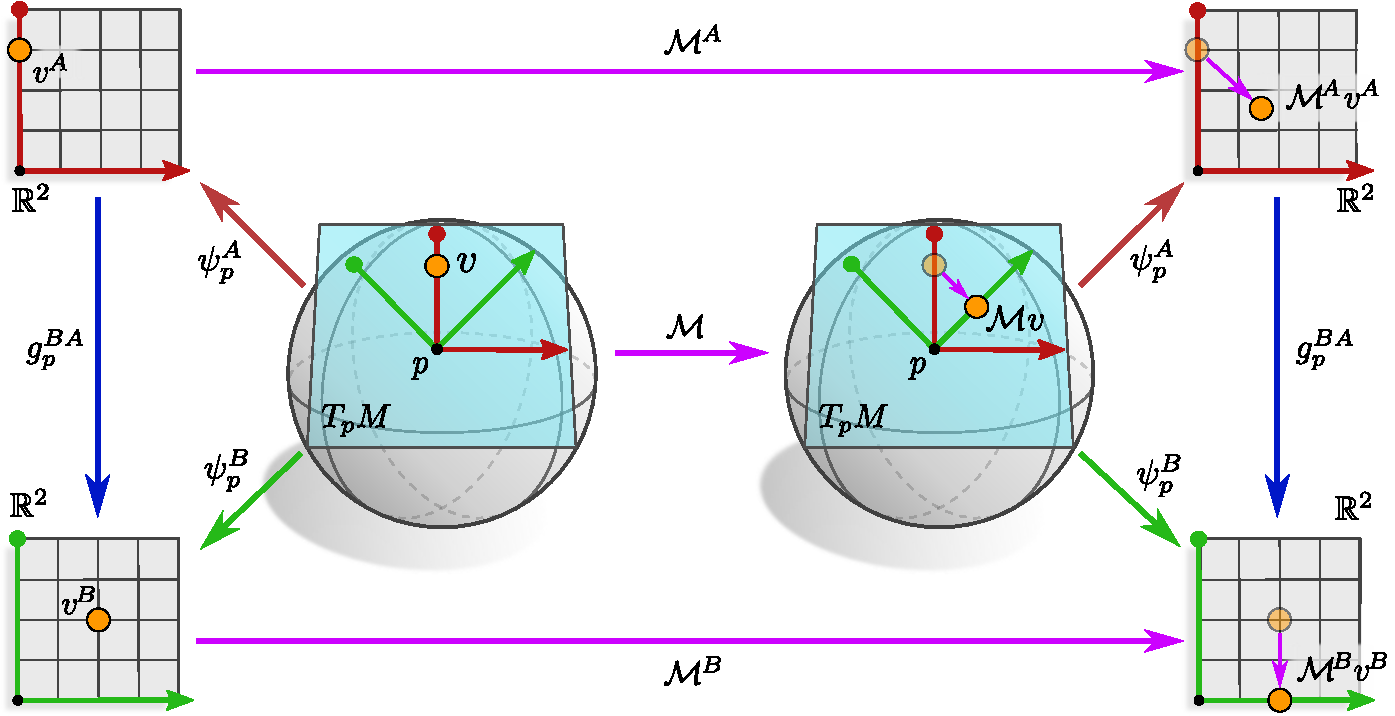
\includegraphics[width=\columnwidth]{figures/gauges_TpM_functions.pdf}
	\vspace*{.5ex}
	\caption{\small
		تفسیر گرافیکی نمودار جابجایی در معادله~\eqref{eq:linear_map_TpM_diagram}.
		یک نگاشت مستقل از مختصات $\mathcal{M}: \TpM \to \TpM$ را می‌توان به طور معادل با توابع $\MAA\!: \R^d \to \R^d$ یا $\MBB\!: \R^d \to \R^d$ \mbox{نسبت به گیج‌های مختلف $\psi_p^A$ یا~$\psi_p^B$} نمایش داد.
		این مختصات‌بندی‌های $\mathcal{M}$ با پیش‌ و پس‌ ترکیب با گیج‌ها در دامنه و دامنه مشترک تعریف می‌شوند، به عنوان مثال، با دنبال کردن فلش‌ها، $\MAA := \psi_p^A \circ \mathcal{M} \circ \big(\psi_p^A\big)^{-1}$.
		در نتیجه، تبدیل‌های گیج $\MBB = g_p^{BA} \MAA \big(g_p^{BA}\big)^{-1}$ بین مختصات‌بندی‌ها توسط یک پیش‌ و پس‌ ترکیب با نگاشت‌های گذار~$g_p^{BA}$ در دامنه و دامنه مشترک داده می‌شوند.
		\emph{همه} کمیت‌ها و نگاشت‌ها در این کار یا مستقل از مختصات خواهند بود (مانند $\mathcal{M}$) یا به روشی مستقل از مختصات در گیج‌های مختلف بیان خواهند شد (مانند $\MAA$ و $\MBB$).
		ما بنابراین باید قوانین تبدیل را برای هر کمیت و تابع تعریف (یا استخراج) کنیم.
	}
	\label{fig:gauge_trafos_functions}
\end{figure}

به عنوان یک مثال ساده برای یک عملیات مستقل از مختصات، بیایید حالت یک \emph{نگاشت خطی} را در نظر بگیریم:
\begin{align}
	\mathcal{M}:\TpM\to \TpM \,.
\end{align}
فرض کنید $v_\text{\lr{in}}\in \TpM$ یک بردار مماس باشد که توسط $\mathcal{M}$ به $v_\text{\lr{out} }= \mathcal{M} v_\text{\lr{in}} \in \TpM$ نگاشت می‌شود.
نگاشت‌های خطی در پیاده‌سازی‌های عددی معمولاً توسط \emph{ماتریس‌های ضریب} مدل می‌شوند که بین \emph{بردارهای ضریب} نسبت به یک انتخاب از چارچوب مرجع نگاشت می‌کنند.
برای دقیق کردن این موضوع، فرض کنید گیج $\psi_p^A$ داده شده باشد به طوری که بردارهای مستقل از مختصات $v_\textup{\lr{in}}$ و $v_\textup{\lr{out}}$ در $\TpM$ با بردارهای ضریب $v_\text{\lr{in}}^A=\psi_p^A(v_\text{\lr{in}})$ و $v_\text{\lr{out}}^A=\psi_p^A(v_\text{\lr{out}})$ در~$\R^d$ نمایش داده شوند.
نگاشت خطی $\mathcal{M}$ در این گیج توسط ماتریس نمایش داده می‌شود:
\begin{align}\label{eq:matrix_trivialization}
	\MAA\ :=\ \psi_p^A \circ \mathcal{M} \circ \big(\psi_p^A\big)^{-1} \ \ \in\ \R^{d\times d}
\end{align}
که تعریف آن توسط نمودار جابجایی زیر بصری‌سازی شده است:
\begin{equation}\label{eq:bundle_morphism_onexone}
	\begin{tikzcd}[row sep=4.em, column sep=4.em]
		\R^d
		\arrow[rrr, pos=.5, rounded corners, to path={
			-- ([yshift=-3.5ex]\tikztostart.south)
			--node[below]{\small$
				\MAA
				$} ([yshift=-3.5ex]\tikztotarget.south)
			-- (\tikztotarget.south)
		}]
		& \TpM  \arrow[r, "\mathcal{M}"]
		\arrow[l, "\psi_p^A"']
		& \TpM  \arrow[r, "\psi_p^A"]
		& \R^d
	\end{tikzcd}
\end{equation}
ماتریس با نگاشت مستقل از مختصات سازگار است زیرا هر دو یکدیگر را نتیجه می‌دهند:
\begin{align}
	\MAA v^A_\text{\lr{in}}
	\ &=\ \pig[ \psi_p^A \circ \mathcal{M} \circ \big(\psi_p^A\big)^{-1} \pig] \circ \pig[ \psi_p^A(v_\text{\lr{in}}) \pig] \notag \\
	\ &=\ \psi_p^A \big( \mathcal{M}\mkern2mu v_\text{\lr{in}} \big) \notag \\
	\ &=\ \psi_p^A (v_\text{\lr{out}}) \notag \\
	\ &=\ v_\text{\lr{out}}^A
\end{align}
البته می‌توان $\mathcal{M}$ را نسبت به هر انتخاب دیگری از گیج $\psi_p^B$ نیز نمایش داد.
ما از معادله~\eqref{eq:components_leftaction} می‌دانیم که بردارهای ضریب در گیج‌های مختلف با $v^B = g_p^{BA} v^A$ مرتبط هستند.
به طور مشابه، $\MBB$ با $\MAA$ توسط تبدیل گیج مرتبط است:
\begin{alignat}{2}\label{eq:matrix_gaugetrafo}
	\MBB
	\ &=&\ \ \psi_p^B \circ\, &\mathcal{M} \circ \big(\psi_p^B\big)^{-1} \notag \\
	\ &=&\ \ \psi_p^B \circ \big(\psi_p^A\big)^{-1} \circ\, &\MAA \circ \psi_p^A \circ \big(\psi_p^B\big)^{-1} \notag \\
	\ &=&\ \ g_p^{BA} &\MAA \big(g_p^{BA}\big)^{-1} \,,
\end{alignat}
که در اینجا هم بر دامنه و هم بر دامنه مشترک عمل می‌کند.%
\footnote{
	تبدیل ضرایب ماتریس از طریق ضرب چپ و راست با $g^{BA}$ و $\big(g^{BA}\big)^{-1}$ به ترتیب، نگاشت خطی را به عنوان یک تانسور از نوع $(1,1)$ شناسایی می‌کند.
}
این قانون تبدیل دوباره سازگار است زیرا تبدیل‌های متقابل یکدیگر را خنثی می‌کنند:
\begin{align}
	\MBB v^B_\text{\lr{in}}
	\ &=\ \pig[ g_p^{BA} \MAA \big(g_p^{BA}\big)^{-1} \pig]\, \pig[ g_p^{BA} v_\text{\lr{in}}^A \pig] \notag \\
	\ &=\ g_p^{BA} \MAA v_\text{\lr{in}}^A \notag \\
	\ &=\ g_p^{BA} v_\text{\lr{out}}^A \notag \\
	\ &=\ v_\text{\lr{out}}^B
\end{align}
تبدیل‌های گیج استخراج شده بنابراین تأیید می‌کنند که تمام محاسبات مختصات‌بندی شده در نهایت مستقل از مختصات هستند.
روابط بین نگاشت مستقل از مختصات و مختصات‌بندی‌های آن توسط نمودار جابجایی زیر خلاصه می‌شود:
\begin{equation}\label{eq:linear_map_TpM_diagram}
	\begin{tikzcd}[column sep=50pt, row sep=25pt, font=\normalsize]
		\R^d
		\arrow[dd, "g_p^{BA}\cdot\ "']
		\arrow[rrr, "\MAA"]
		& &[-2ex] &
		\R^d
		\arrow[dd, "\ g_p^{BA}\cdot"]
		\\
		&
		\TpM
		\arrow[ul, "\psi_p^A"]
		\arrow[dl, "\psi_p^B"']
		\arrow[r, "\mathcal{M}"]
		&
		\TpM
		\arrow[ur, "\psi_p^A"']
		\arrow[dr, "\psi_p^B"]
		\\
		\R^d
		\arrow[rrr, "\MBB"']
		& & &
		\R^d
	\end{tikzcd}
\end{equation}
که در شکل~\ref{fig:gauge_trafos_functions} به صورت گرافیکی تفسیر شده است.

در عمل نمی‌توان نگاشت خطی مستقل از مختصات $\mathcal{M}$ را به صورت عددی بدون اشاره به یک انتخاب مختصات‌بندی پیاده‌سازی کرد.
با این حال، وجود آن تنها در صورتی (و تنها در صورتی) دلالت دارد که مختصات‌بندی‌های آن همانطور که در معادله~\eqref{eq:matrix_gaugetrafo} مشخص شده است به یکدیگر مربوط باشند، که تضمین می‌کند رفتار تبدیل صحیح ضرایب بردار ورودی و خروجی در معادله~\eqref{eq:components_leftaction} حفظ می‌شود.


\subsubsection{گروه‌های ساختار، \textit{$G$}-ساختارها و \textit{$G$}-اطلس‌ها}
\label{sec:local_G-structure_G-atlas}

ما بعداً از شبکه‌های عصبی می‌خواهیم که به روشی مستقل از مختصات عمل کنند، یعنی ما تقاضا می‌کنیم که استنتاج آن‌ها مستقل از انتخاب‌های دلخواه چارچوب‌های مرجع باشد.
این سؤال را مطرح می‌کند که انتخاب چارچوب‌های مرجع در یک منیفولد تا چه حد دلخواه است.
در بخش‌های~\ref{sec:gauges_gauge_trafos} و~\ref{sec:gauges_TpM_functions} قبلی ما هر انتخاب ممکن از گیج یا چارچوب مرجع را مجاز می‌دانستیم، که بنابراین توسط تبدیل‌های گیج با مقدار کلی $\GL{d}$ مرتبط بودند.
با این حال، در بسیاری از کاربردها، منیفولد دارای ساختار اضافی است که امکان تشخیص یک \emph{زیرمجموعه ارجح از چارچوب‌های مرجع} یا گیج‌ها را می‌دهد که توابع گذار آن‌ها مقادیری در یک \emph{گروه ساختار کاهش یافته} $G\leq\GL{d}$ می‌گیرند.
چنین ساختارهای هندسی ـ یا بلکه خود زیرمجموعه‌های چارچوب‌های مرجع ترجیحی، که اطلاعات معادل را کدگذاری می‌کنند ـ به عنوان \emph{$G$-ساختارها} نامیده می‌شوند.


$G$-ساختارها با در نظر گرفتن چند مثال خاص بهتر درک می‌شوند.
لیست زیر چنین مثال‌هایی را ارائه می‌دهد که بر اساس گروه ساختار $G \leq \GL{d}$ طبقه‌بندی شده‌اند:
\begin{itemize}[leftmargin=9.4ex]
	\item[$\OO{d}$:]
	\emph{ساختار متریک} یک منیفولد ریمانی را در نظر بگیرید، که امکان اندازه‌گیری فواصل و زوایا را می‌دهد، و بنابراین تشخیص چارچوب‌های متعامد را، یعنی آن چارچوب‌هایی که شرط $\eta(e_i,e_j) = \delta_{ij}$ را برای هر $i,j=1,\dots,d$ برآورده می‌کنند.
	به طور متناظر، یک متریک ریمانی امکان صحبت در مورد گیج‌های ایزومتریک $\psi_p^A$ را می‌دهد، که متریک $\R^d$ را با متریک~$\TpM$ شناسایی می‌کنند، یعنی شرط $\eta(v,w) = \langle \psi_p^A(v),\, \psi_p^A(w) \rangle_{\R^d}$ را برای هر $v,w \in \TpM$ برآورده می‌کنند.
	از آنجا که چارچوب‌های متعامد و گیج‌های ایزومتریک تا چرخش‌ها و بازتاب‌ها تعریف می‌شوند، هر تبدیل گیجی بین آن‌ها مقادیری در گروه متعامد~$\OO{d}$ خواهد گرفت، که آن زیرگروه از $\GL{d}$ است که زوایا و فواصل را حفظ می‌کند.
	\item[$\operatorname{GL}^+(d)$:]
	به طور مشابه، یک \emph{جهت‌گیری} منیفولد چارچوب‌های راست‌گرد را از چپ‌گرد و گیج‌های حفظ‌کننده جهت‌گیری را از گیج‌های معکوس‌کننده جهت‌گیری متمایز می‌کند.
	تبدیل‌های گیج بین چارچوب‌های یک دست‌پری داده شده مقادیری در $\operatorname{GL}^+(d)$ می‌گیرند، یعنی آن زیرگروه از $\GL{d}$ که جهت‌گیری‌ها را حفظ می‌کند.
	\item[$\SO{d}$:]
	با هم، یک \emph{متریک و جهت‌گیری} داده شده، چارچوب‌های متعامد با جهت‌گیری خاصی را مشخص می‌کنند.
	تبدیل‌های گیج بین چنین چارچوب‌هایی تضمین شده‌اند که در زیرگروه~$\SO{d}$ از $\GL{d}$ قرار گیرند.
	\item[$\{e\}$:]
	یک \emph{میدان چارچوب هموار سراسری} یک $\{e\}$-ساختار را در $M$ تعریف می‌کند.
	در این حالت تنها یک چارچوب متمایز در هر موقعیت وجود دارد، به طوری که تبدیل‌های گیج در گروه بدیهی ${\{e\} \leq \GL{d}}$ قرار می‌گیرند.
	\item[$\GL{d}$:]
	اگر هیچ ساختار اضافی تحمیل نشود، \emph{هر} چارچوب مرجع فضاهای مماس به همان اندازه معتبر است.
	تبدیل‌های گیج در این حالت نگاشت‌های خطی معکوس‌پذیر عمومی در $\GL{d}$ هستند و $G$-ساختار مربوطه فقط بندل چارچوب $\FM$ است.
\end{itemize}


\begin{samepage}
	موضوع مشترک در این مثال‌های انگیزشی این است که همه آن‌ها با موارد زیر تعریف می‌شوند:
	\begin{enumerate}
		\item یک زیرمجموعه (که به صورت فضایی هموار تغییر می‌کند) از چارچوب‌های مرجع متمایز،
		\item یک زیرمجموعه مربوطه از گیج‌های ترجیحی و
		\item یک زیرگروه $G \leq \GL{d}$ از تبدیل‌های گیج که مفهوم متمایز چارچوب‌ها و گیج‌ها را حفظ می‌کنند.
	\end{enumerate}
\end{samepage}
چنین زیرمجموعه‌هایی از چارچوب‌های مرجع که به صورت هموار تغییر می‌کنند به عنوان \emph{$G$-ساختارها}~$\GM$ بر روی~$M$ نامیده می‌شوند
و گروه~$G$ به عنوان \emph{گروه ساختار} (کاهش یافته) نامیده می‌شود ـ برای تعریفی دقیق‌تر به بخش~\ref{sec:G_associated_bundles} مراجعه کنید.%
\footnote{
	به طور رسمی، $\GM$ به عنوان یک زیربندل اصلی $G$ از بندل چارچوب $\FM$ تعریف می‌شود، که یک بندل اصلی $\GL{d}$ است.
}
فرآیند مشخص کردن یک $G$-ساختار به عنوان \emph{کاهش گروه ساختار} از $\GL{d}$ به~$G$ شناخته می‌شود.
یک اطلس ${\mathscr{A}^G = \big\{\! \big(U^X, \psi^X\big) \!\big\}_{X\in \mathfrak{X}}}$ به عنوان $G$-\emph{اطلس} نامیده می‌شود اگر تمام توابع گذار آن:
\begin{align}\label{eq:transition_fct_local_def_21_G_atlas}
	g^{BA}\!:\, U^A\cap U^B\to G, \quad p \mapsto g_p^{BA} := \psi_p^B \circ \left(\psi_p^A\right)^{-1}
\end{align}
در یک گروه ساختار کاهش یافته~$G \leq \GL{d}$ قرار گیرند (مقایسه کنید با معادله~\eqref{eq:transition_fct_local_def_21}).
رابطه بین چارچوب‌های مرجع و گیج‌ها در معادله~\eqref{eq:framefield_gauge_equivalence} دلالت دارد بر اینکه هر $G$-اطلس یک $G$-ساختار مربوطه را کدگذاری می‌کند.


انتخاب‌های متعددی از $G$-ساختارها ممکن است برای یک گروه ساختار $G$ داده شده وجود داشته باشند.
برای ارتباط با مثال‌های بالا:
متریک‌های ریمانی مختلف، زیرمجموعه‌های متفاوتی از چارچوب‌های مرجع را به عنوان متعامد مشخص می‌کنند، یعنی آن‌ها با ساختارهای $\OO{d}$ مختلف $\OM$ مطابقت دارند.
بنابراین انتخاب یک متریک معادل انتخاب یک ساختار $\OO{d}$ است.
به طور مشابه، انتخاب‌های مختلف جهت‌گیری یک منیفولد قابل جهت‌گیری، مجموعه متفاوتی از چارچوب‌ها را به عنوان راست‌گرد مشخص می‌کنند.
بنابراین دو انتخاب ممکن جهت‌گیری با دو انتخاب ممکن از ساختارهای $\operatorname{GL}^+(d)$ ($\operatorname{GL}^+\mkern-5muM$) مطابقت دارند.
ساختارهای $\SO{d}$ ($\SOM$) ممکن است در انتخاب جهت‌گیری و متریک هر دو متفاوت باشند.
مثال دیگر ساختار $\{e\}$ $\eM$ است.
آن‌ها اجازه تبدیل‌های گیج (غیربدیهی) را نمی‌دهند و بنابراین با انتخاب میدان‌های چارچوب هموار سراسری در $M$ مطابقت دارند.
جدول~\ref{tab:G_structures} مثال‌های بیشتری از گروه‌های ساختار~$G$ و $G$-ساختارهای مربوطه را ارائه می‌دهد.


\begin{table}
	\centering
	\renewcommand\arraystretch{1.1}
	\small
	\begin{latin}
		\begin{tabular}{cll}
			\toprule
			structure group $G\leq\GL{d}$ & $G$-structure $\GM$			& equivalent structure on $M$		\\[.25ex]
			\midrule
			$\operatorname{GL}^+(d)$	& positively oriented frames			& orientation of $M$			\\
			$\operatorname{SL}(d)$		& unit volume frames				& volume form				\\
			$\operatorname{CO}(d)$		& conformal frames				& ---					\\
			$\operatorname{Sp}(d)$		& symplectic frames				& ---					\\
			$\operatorname{O}(d)$		& orthonormal frames				& Riemannian metric			\\
			$\operatorname{O}(d-n,\,n)$	& pseudo-orthonormal frames			& pseudo-Riemannian metric		\\
			$\operatorname{SO}(d)$		& positively oriented orthonormal frames	& Riemannian metric + orientation	\\
			$\{e\}$				& parallelization (global frame field)	& ---					\\[.25ex]
			\bottomrule
		\end{tabular}
	\end{latin}
	\vspace*{2ex}
	\caption{
		مثال‌هایی از $G$-ساختارها $\GM$ بر روی $M$ و گروه‌های ساختار کاهش‌یافته مربوطه~$G\leq\GL{d}$.
		یک~$G$-ساختار به عنوان یک زیرمجموعه هموار متغیر از چارچوب‌های مرجع (یک زیربندل اصلی $G$ از بندل چارچوب $\FM$) تعریف می‌شود، که در آن چارچوب‌های هر فضای مماس به صورت متقابل توسط تبدیل‌های گیج با مقدار $G$ مرتبط هستند.
		در حالی که این تعریف نسبتاً انتزاعی است، امکان مشاهده بسیاری از ساختارهای هندسی در~$M$ را به روشی یکپارچه فراهم می‌کند.
		به عنوان مثال، یک متریک ریمانی در~$M$ امکان تشخیص چارچوب‌های متعامد را می‌دهد.
		برعکس، مشخص کردن متعامد بودن به طور منحصر به فرد یک متریک را نتیجه می‌دهد.
		بنابراین یک متریک ریمانی و یک ساختار متعامد با یکدیگر معادل هستند.
		به طور مشابه، یک تناظر یک به یک بین فرم‌های حجم و چارچوب‌های واحد حجم وجود دارد.
		توجه داشته باشید که انتخاب یک گروه ساختار $G$ به طور منحصر به فرد یک $G$-ساختار را مشخص نمی‌کند.
		به عنوان مثال، متریک‌های ریمانی مختلف می‌توانند به عنوان ساختار $\OO{d}$، فرم‌های حجم مختلف به عنوان ساختار $\operatorname{SL}(d)$ یا میدان‌های چارچوب سراسری مختلف به عنوان ساختار $\{e\}$ انتخاب شوند.
		\CNN{}های مستقل از مختصات برای رعایت یک $G$-ساختار داده شده طراحی شده‌اند ـ اینکه کدام ساختار خاص است به وظیفه یادگیری بستگی دارد.
	}
	\label{tab:G_structures}
\end{table}


کاهش گروه ساختار به $G$، یعنی وجود یک $G$-ساختار، ممکن است توسط توپولوژی منیفولد مسدود شود.
این دلالت دارد بر اینکه یک \emph{"گروه ساختار کاهش‌ناپذیر"} وجود دارد که فراتر از آن ابهام چارچوب‌های مرجع را نمی‌توان بدون نقض فرض همواری (یا حتی پیوستگی) $G$-ساختار برطرف کرد.
به عنوان مثال، نوار موبیوس در شکل~\ref{fig:mobius_conv_gauges} غیرقابل جهت‌گیری است. این بدان معنی است که یک تعریف هموار و سراسری سازگار از دست‌پری چارچوب و در نتیجه ساختار $\{e\}$ (میدان چارچوب هموار سراسری) را نمی‌پذیرد.
همانطور که در شکل~\ref{fig:mobius_conv_gauges} بصری‌سازی شده است، یک $G$-اطلس از گیج‌ها که نوار موبیوس را پوشش می‌دهد، به طور ناگزیر نیازمند یک بازتاب در یکی از نگاشت‌های گذار خواهد بود، که به معنای یک گروه ساختار کاهش‌ناپذیر $G=\Flip$ است.
\CNN{}های مستقل از مختصات بر روی نوار موبیوس بنابراین حداقل باید تناوب‌پذیر بازتابی باشند.
به طور مشابه، گروه ساختار کره را نمی‌توان فراتر از $G=\SO{2}$ کاهش داد.
\CNN{}های کروی هموار بنابراین لزوماً بر پایه کرنل‌های محلی تناوب‌پذیر چرخش هستند.


توجه داشته باشید که \emph{هر} منیفولد (دیفرانسیل‌پذیر) با \emph{برخی} $G$-ساختار همراه است.
به عنوان مثال، یک منیفولد دیفرانسیل‌پذیر خام دارای یک ساختار $\GL{d}$ (حاوی هر چارچوب ممکن) است، یک منیفولد ریمانی یک ساختار $\OO{d}$ دارد و $\R^d$ به طور کانونی با یک ساختار $\{e\}$ مجهز شده است که در شکل~\ref{fig:frame_field_automorphism_1} بصری‌سازی شده است.
ما بنابراین بدون از دست دادن کلیت، اصطلاح "استقلال از مختصات" را به \emph{استقلال از مختصات} $\GM$ تصحیح خواهیم کرد، یعنی استقلال نسبت به انتخاب چارچوب‌های مرجع در $G$-ساختار داده شده در~$M$.
در طول این کار ما فرض خواهیم کرد که گیج‌ها بخشی از یک $G$-اطلس هستند:
\begin{align}\label{eq:G_atlas_dfn}
 	\ \ p\in U^A\cap U^B \,,
 	\ \ \ \psi_p^A, \psi_p^B \in \mathscr{A}^G,
 	\quad \textup{برای هر}
	\quad g_p^{BA} \in G 
	\quad\ \textup{چنان که} \quad
	\mathscr{A}^G \,=\, \big\{\! \big(U^X, \psi^X\big) \!\big\}_{X\in \mathfrak{X}}
\end{align}
مطابق با $G$-ساختار داده شده.
هر کمیت یا تابع می‌تواند نسبت به هر گیجی از این اطلس بیان شود%
\footnote{
	این یک گزاره غیربدیهی است زیرا هر کمیتی را نمی‌توان نسبت به چارچوب‌های مرجع دلخواه مرتبط با $\GL{d}$ بیان کرد.
	به عنوان مثال، میدان‌های ویژگی که در بخش~\ref{sec:feature_fields} معرفی شده‌اند، تنها تبدیل‌های گیج با مقدار $G$ را می‌پذیرند و بنابراین تنها نسبت به چارچوب‌های ترجیحی در~$\GM$ تعریف می‌شوند.
	به عنوان یک مثال شهودی، \CNN{}های سنتی (غیرتناوب‌پذیر) در $\R^d$ را در نظر بگیرید که نسبت به ساختار $\{e\}$ کانونی $\R^d$ استخراج می‌شوند و اطلاعاتی در مورد پاسخ‌های کرنل نسبت به سایر چارچوب‌های مرجع را حمل \emph{نمی‌کنند}.
}،
و مختصات‌بندی‌ها در گیج‌های مختلف به طور منحصر به فرد توسط یک تبدیل گیج با مقدار $G$ مرتبط هستند.
با تضمین استقلال از مختصات همه ساختارها، آن‌ها همیشه با همتایان مستقل از مختصات خود مطابقت خواهند داشت، که ما نظریه سراسری را بر حسب آن‌ها در بخش‌های~\ref{sec:bundles_fields}، \ref{sec:gauge_CNNs_global} و~\ref{sec:isometry_intro} فرمول‌بندی خواهیم کرد.